\documentclass{article}
\usepackage{amsmath}
\usepackage{amssymb}
\usepackage{graphicx}
\usepackage{hyperref}
\usepackage[version=4]{mhchem}


\begin{document}
(2005 AIME II Problem 14) In \(\triangle A B C, A B=13, B C=15\), and \(C A=\) 14. Point \(D\) is on \(B C\) with \(C D=6\). Point \(E\) is on \(B C\) such that \(\angle B A E=\angle C A D\).

Given that \(B E=p / q\), where \(p\) and \(q\) are relatively prime positive integers, find \(q\).\\
Solution: 463.\\
Draw \(B F / / A C\) to meet the extension of \(A E\) at \(G\) and \(A D\) at \(F\).\\
We know that \(A C / / B F\). So \(\triangle A D C \sim \triangle F D B\) (figure 1). \(\frac{A C}{B F}=\frac{D C}{B D} \Rightarrow\)

\[
\frac{14}{B F}=\frac{6}{9} \quad \Rightarrow \quad B F=\frac{14 \times 9}{6}=21
\]

We know that \(\angle B A G=\angle B F A=\alpha\) and \(\angle A B G=\angle A B F\) (figures 2 and 3). So \(\triangle A B G \sim \triangle A B F . \frac{A B}{B F}=\frac{B G}{A B} \Rightarrow \quad \frac{13}{21}=\frac{B G}{13} \Rightarrow \quad B G=\frac{169}{21}\)\\
We know that \(A C / / B F\). So \(\triangle B G E \sim \triangle C A E\) (figure 4).\\
\(\frac{B G}{A C}=\frac{B E}{C E}\)\\
\(\Rightarrow \quad \frac{\frac{169}{21}}{14}=\frac{x}{15-x}\)\\
\(\Rightarrow \quad x=\frac{2535}{463}\).

The answer is 463 .\\
\centering
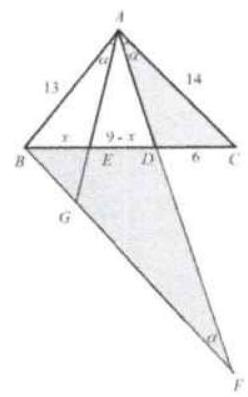
\includegraphics[width=\textwidth]{images/121(1).jpg}\\
Figure 1\\
\centering
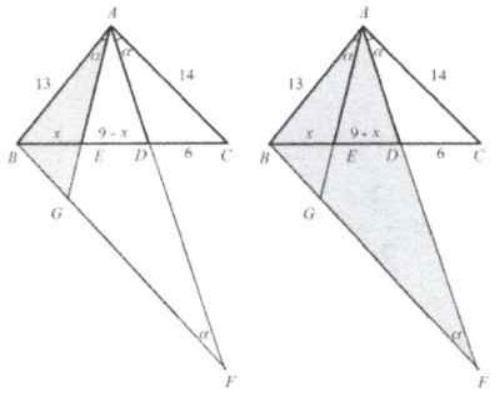
\includegraphics[width=\textwidth]{images/121(3).jpg}\\
Figures 2 and 3\\
\centering
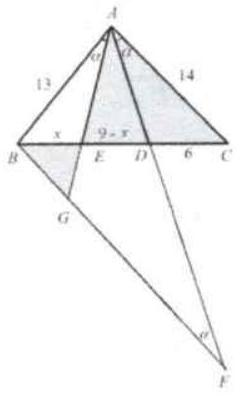
\includegraphics[width=\textwidth]{images/121.jpg}\\
Figure 4


\end{document}
